\graphicspath{{content/appendices/figures/}}

\chapter{Preliminary Experiments}

\vfill
\begin{figure}[!htbp]
    \centering% width=1, they do not fit on a single page
    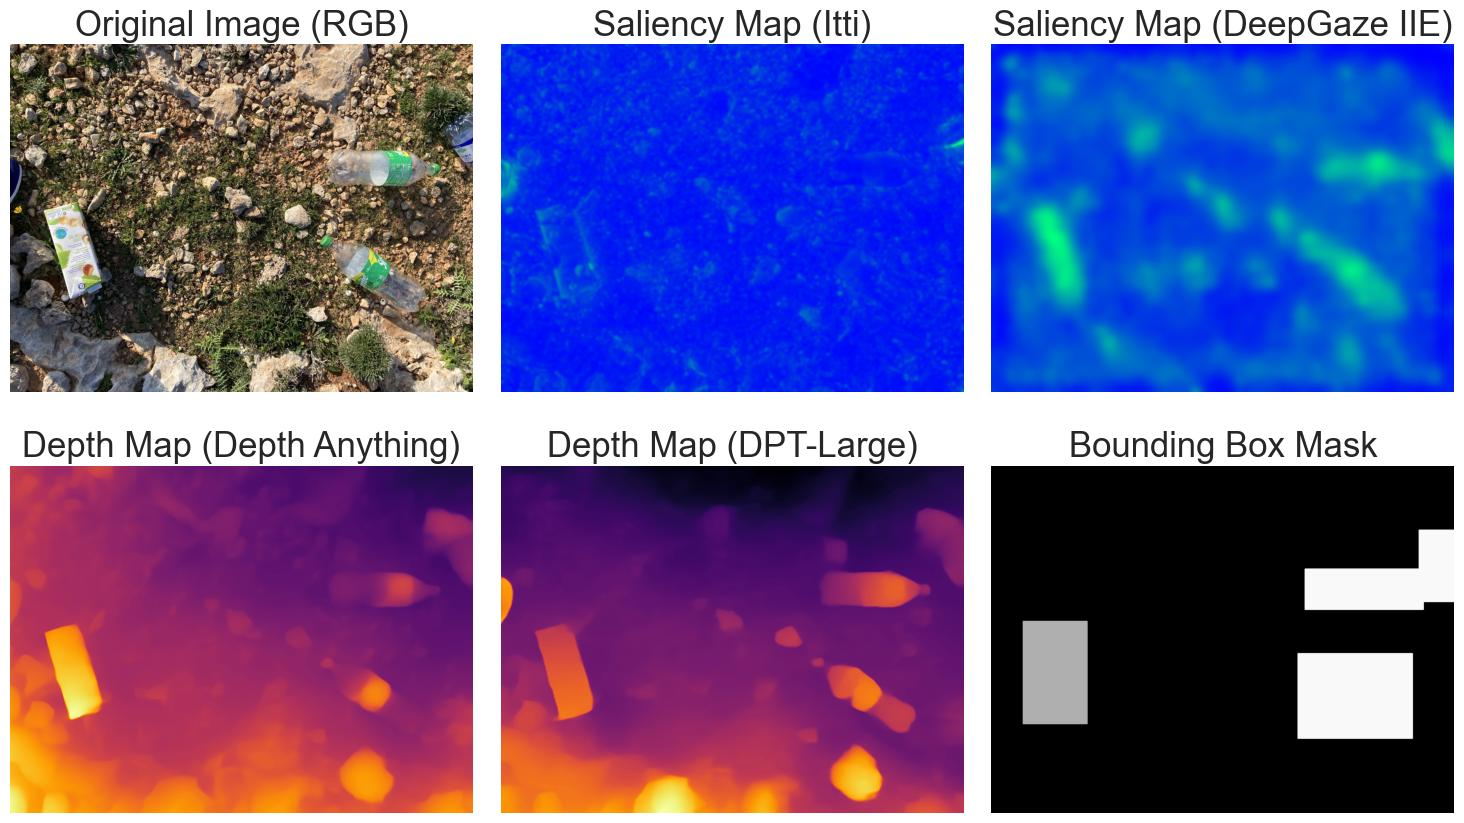
\includegraphics[width=0.9\columnwidth]{privileged_information_soda_01m.png}
    \caption{Examples of generated privileged information derived from a selected image in the SODA dataset \cite{soda_dataset}. The original image (RGB, three-channel) is shown alongside corresponding single-channel representations, each depicting a distinct form of privileged information that may be considered during training.}
    \label{fig:channels}
\end{figure}
\vfill
\vfill
\begin{figure}[!htbp]
    \centering
    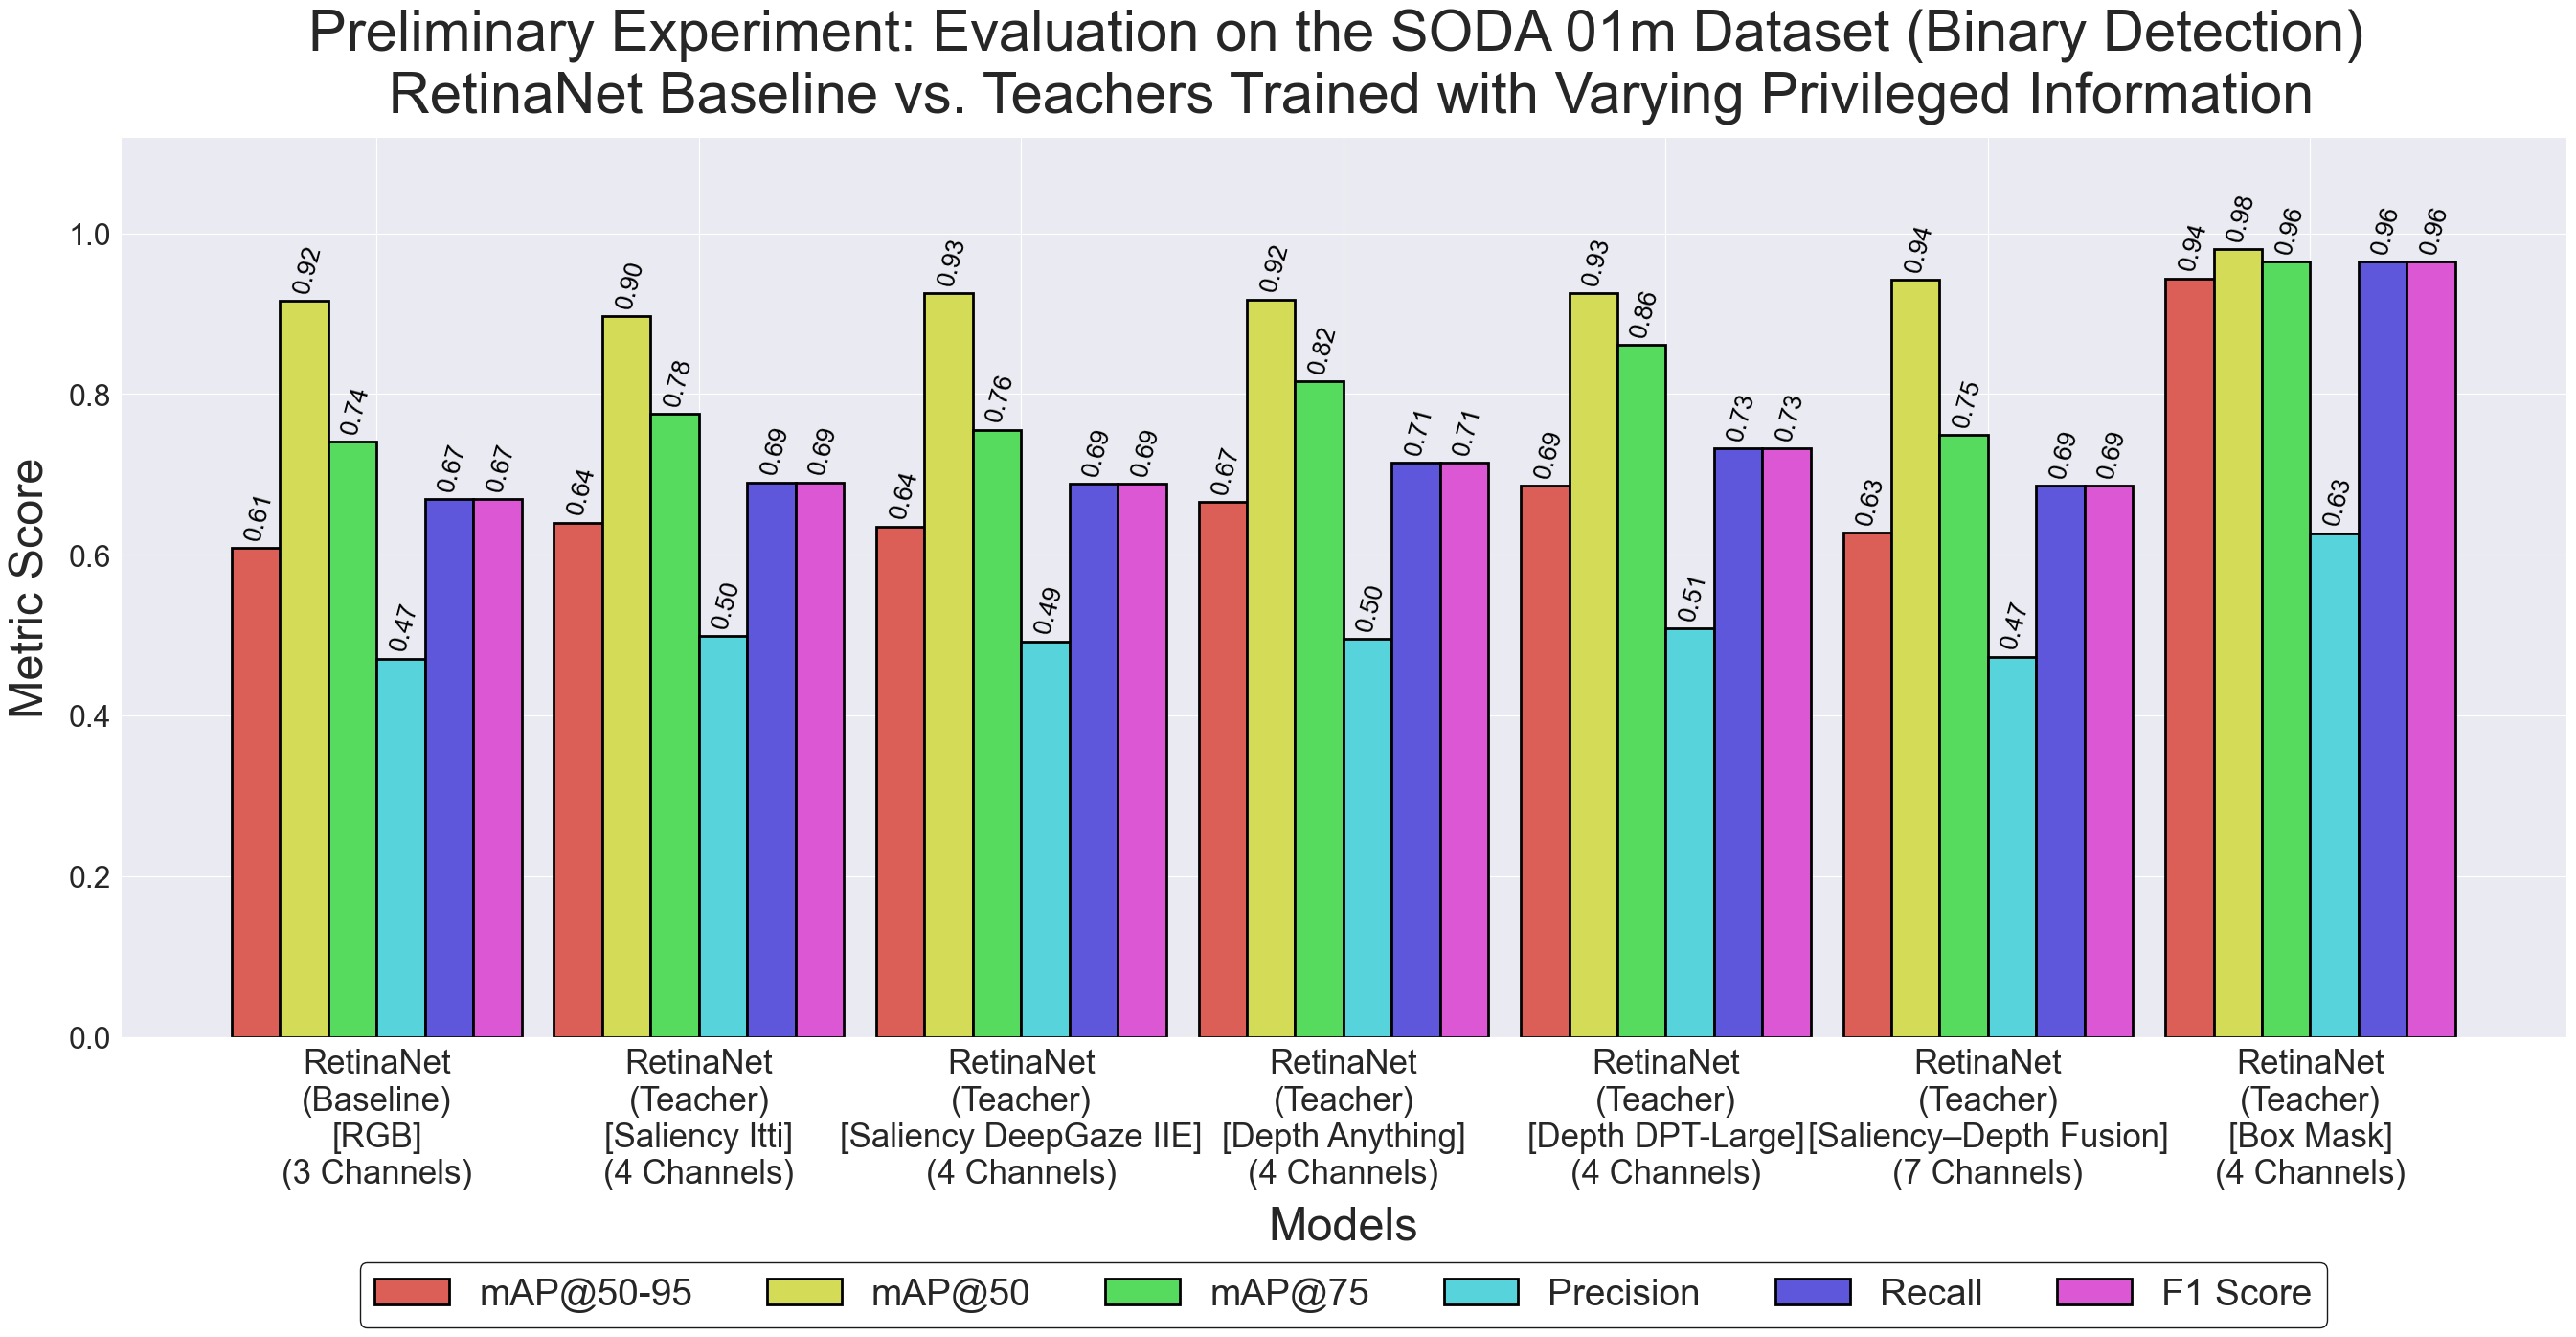
\includegraphics[width=0.9\columnwidth]{Preliminary Experiment Privileged Information Selection.png}
    \caption{Evaluation results on the SODA 01m altitude dataset for the binary litter detection task. The figure compares the RetinaNet baseline model with various teacher models trained using different forms of privileged information. Among the tested variants, the model utilising Bounding Box Mask privileged information yielded the most notable improvement, while other types of privileged information resulted in only marginal gains relative to the baseline.}
    \label{fig:preliminary_privileged}
\end{figure}
\vfill